\section{Vanishing and Exploding Gradients}
\begin{frame}{Vanishing and Exploding Gradients}
  \small
  \textbf{Backpropagation Through Time (BPTT)} spreads gradients across many time steps.
  
  \vspace{1em}
  {\color{red}\textbf{Vanishing Gradients:}}
  \begin{align*}
    \left\| \frac{\partial \mathcal{L}}{\partial h_t} \right\| \rightarrow 0
  \end{align*}
  \begin{itemize}
    \item[\textcolor{red}{$\blacktriangleright$}] Early layers barely learn
    \item[\textcolor{red}{$\blacktriangleright$}] Forget long-term dependencies
  \end{itemize}
  \vspace{0.5em}
  {\color{blue}\textbf{Exploding Gradients:}}
  \begin{align*}
    \left\| \frac{\partial \mathcal{L}}{\partial h_t} \right\| \rightarrow \infty
  \end{align*}
  \begin{itemize}
    \item[\textcolor{red}{$\blacktriangleright$}] Unstable updates, diverging weights
  \end{itemize}
\end{frame}

\begin{frame}{Solving for vanishing or exploding gradients}
  \begin{itemize}
    \item Identity RNN with ReLU activation
    \hfill
    \(
      \left[
        \begin{array}{ccccc}
          1 & 0 & 0 & 0 & 0 \\
          0 & 1 & 0 & 0 & 0 \\
          0 & 0 & 1 & 0 & 0 \\
          0 & 0 & 0 & 1 & 0 \\
          0 & 0 & 0 & 0 & 1 \\
        \end{array}
      \right]
    \)
    \item Gradient clipping
    \item Skip connections
      \begin{center}
        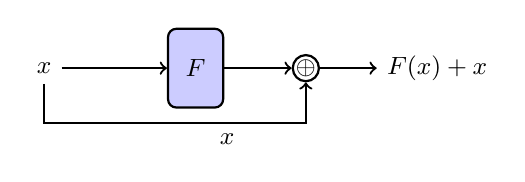
\begin{tikzpicture}[every node/.style={font=\small},thick,scale=1.0]
          % Nodes
          \node[left] (x) at (0,1) {$x$};
          \node[draw,rounded corners=3pt,fill=blue!20,minimum width=0.7cm,minimum height=1cm] (block) at (1.7,1) {$F$};
          \node[circle,draw,inner sep=0pt,minimum size=0.3cm] (plus) at (3.1,1) {$\oplus$};
          \node[right] (out) at (4,1) {$F(x)+x$};

          % Arrows: forward
          \draw[->,thick] (x) -- (block);
          \draw[->,thick] (block) -- (plus);
          \draw[->,thick] (plus) -- (out);

          % Skip connection: carries x unchanged past the block
          \draw[->,thick] (x) |- (2.1,0.3) -| (plus);
          \node[below] at (2.1,0.3) {$x$};

        \end{tikzpicture}
      \end{center}
  \end{itemize}
\end{frame}

\begin{frame}{Gradient Clipping}
  Exploding gradients are a problem of \emph{magnitude}, so they have a cheap fix: after
  backpropagation, rescale the gradient whenever it grows past a threshold $\tau$.
  \vspace{0.3em}
  \begin{align*}
    g \leftarrow \frac{\partial \mathcal{L}}{\partial \theta},
    \qquad \text{if } \|g\| > \tau \quad\text{then}\quad g \leftarrow \frac{\tau}{\|g\|}\, g
  \end{align*}
  \vspace{-0.3em}
  \begin{itemize}
    \item The rescaling uses the norm of the gradient over \emph{all} parameters at once, so the
      update \emph{direction} is preserved and only its length is capped.
    \item $\tau$ is a hyperparameter. Pascanu et al.\ (2013) suggest setting it from the average
      gradient norm observed over a stable stretch of training.
    \item It stops one bad batch from destroying the weights, but it does \emph{not} address
      vanishing gradients: rescaling a gradient that has already decayed recovers no information
      about distant time steps. That is what gating is for.
  \end{itemize}
\end{frame}

\begin{frame}{RNN tradeoffs}
  \textbf{RNN Advantages}
  \begin{itemize}
    \item Can process any length input.
    \item Computation for step t can (in theory) use information from many steps back.
    \item Model size doesn’t increase for longer input.
    \item Same weights applied on every timestep, so there is symmetry in how inputs
    are processed.
    \end{itemize}
    \textbf{RNN Disadvantages}
    \begin{itemize}
      \item Recurrent computation is slow
      \item In practice, difficult to access information from many steps back
      \end{itemize} 
\end{frame}
